%!TEX root = main.tex

\section{Spacecraft System Design}
\label{sec:spacecraftsystemdesign}
The intrinsic characteristic of the HT to GEO leads to various spacecraft's system configurations, i.e., the chemical propellant spent during the CP segment changes for each switching orbit, and so does the electric phase. One of the key feature of this work consists in formulating a system design practice for the HTs family.

The payload to deliver in GEO, whatever of the trajectory would be, is a generic communication payload. The power required by a typical communication satellites in GEO\footnote{At the time of writing, operative communication satellites are more than 400(\emph{UCS Satellite Database}) source.} is high. This can be used used to feed the electric thruster during the transfer. The linear regression
%
\begin{equation}
m_{\scriptstyle{{pl}}}= 0.0578 P{_{pl}} + 176.7125
\label{eq:masspayload}
\end{equation}
%
describes the properties of the payload ($m_{\scriptstyle{{pl}}}$ and $P{_{pl}}$ are the payload mass and power, respectively). Eq.\ \eqref{eq:masspayload} is obtained through a statistical analysis of current and future communication payloads (see \tablename\ref{tab:masspower}).
%
\begin{table}[htp]
\footnotesize
\centering
\caption{\textbf{Power and Mass of GEO payloads}}
\label{tab:masspower}
%\caption*{Data retrieved from \cite{atk-web,nasa-web,eoportal-web,sstl-web,ohb-web}.}
\begin{threeparttable}
\begin{tabular}{ccc}
\toprule
\toprule
Mass&Power&Name\\
$\si{\kilo\gram}$&$\si{\watt}$&\\
\midrule
$200$&$450$& \textit{SSTL}-600$^{\dagger}$\\
$300$&$2500$&\textit{GMP-A}$^{\dagger}$\\
$400$&$2500$&\textit{GMP-T}s$^{\dagger}$\\
$300$&$3000$&SmallGEO$^{\star}$\\
$350$&$3500$&\textit{GMP-T}m$^{\dagger}$\\
$450$&$4000$&\textit{GMP-T}$^{\dagger}$\\
$500$&$5000$&\textit{702-SP}$^{\ddagger}$\\
$400$&$6000$&SmallGEO \textit{FAST}$^{\star}$\\
$400$&$6500$&Insat 3000$^{\otimes}$\\
$700$&$7000$&\textit{GMP-TL}$^{\dagger}$\\
$800$&$8000$&GeoStar 3$^{\otimes}$\\
$600$&$8000$&SmallGEO \textit{FLEX}$^{\star}$\\
$1200$&$18000$& Alphabus$^{\ddagger}$\\
\bottomrule      
\bottomrule  
\end{tabular}
\begin{tablenotes}
\footnotesize
\item[$\dagger$]\url{http://www.sstl.co.uk}
\item[$\star$]\url{https://www.ohb-system.de}
\item[$^{\ddagger}$]\url{https://www.directory.eoportal.org}
\item[$^{\otimes}$]\url{http://www.space.skyrocket.de/doc_sat/osc_star-3.htm}
\end{tablenotes}
\end{threeparttable}
\end{table}
%
\\Concerning the spacecraft bus design, it is assumed that there are trajectory-independent subsystems, which are detached from the hybrid transfer performances, and trajectory-dependent subsystems that rely on the present path followed.
This distinction is presented in 
\tablename\ref{tab:spacecraftbusforgeomission}.
\begin{table*}[htp]
\centering
\caption{\textbf{Spacecraft Bus for HTs to GEO}}
\label{tab:spacecraftbusforgeomission}
\small
\begin{tabular}{*{2}{l}}
\toprule
\toprule
Trajectory-independent&Trajectory-dependent\\
\midrule
Attitude and Orbital Control System&EP system\\
On-Board Data Handling&Power Generation System\\
Structural System&CP system\\
Thermal Control System&\\
Telemetry,Tracking and Command System&\\
\bottomrule
\bottomrule
\end{tabular} 
\end{table*}
Trajectory-dependent subsystems are modeled, while the other ones are lumped as having a cumulated mass and power demand of $800~\si{\kilo\gram}$ and $682~\si{\watt}$, respectively~\cite{tesisimo}.
\subsection{Electric Propulsion System}
The tasks of the Electric Propulsion System consist in accomplishing both the orbit raising and the secondary maneuver for all the HTs but for the FCT, where the primary maneuvers are managed with the CP. 

In order to pursuing these aims, in this work three models of Hall Effect Thruster (HET) fed by \emph{Xenon} \cite{szabo2013eight,esa-prof,Hofer:2006aa} are available to perform the HT towards GEO (see \tablename\ref{tab:propertiesofthehetinvestigated}). They are selected because their wide operative envelopes, which guarantee a dual-operation mode. 
This capability allows the thrusters to meet the requirements of high-thrust\footnote{High-thrust for the EP sector.} for orbit raising, when the electric input power is fed with a low voltage, and high specific impulse for on-orbit maneuvers, when the electric input power is fed with a high voltage. Furthermore, HETs represent a good compromise between performance and system properties.
%
\begin{table}[htp]
\centering
\caption{\textbf{Properties of the HETs investigated}}
\label{tab:propertiesofthehetinvestigated}
\footnotesize
\begin{threeparttable}
\begin{tabular}{lcccccc}
\toprule
\toprule
\multirow{3}*{Model HET} & \multicolumn{2}{c}{Power} &\multicolumn{2}{c}{Voltage}&mass&\multirow{3}*{\textit{FP}$^{\dagger}$}\\
&$P_{min}$&$P_{max}$&$\si\volt_{min}$&$\si\volt_{max}$&\si{\kilo\gram}&\\
\cmidrule(lr){2-5}
&$\si{\kilo\watt}$&$\si{\kilo\watt}$&\si\volt&\si\volt&[-]\\
\midrule
\textit{BPT}~4000&$1.15$&$4.91$&200&400&12.3&YES\\
\textit{PPS}~5000&$3.00$&$6.00$&300&800&12&NO\\
\textit{BHT}~8000&$2.00$&$8.00$&200&400&19.2&NO\\
\bottomrule
\bottomrule
\end{tabular}
\begin{tablenotes}
\small
\item[$\dagger$] Flight Proven
\end{tablenotes}
\end{threeparttable}
\end{table}
%
The considered Power Processing Unit (PPU) \cite{Hofer:2006aa,duchemin2011electric} are cataloged in \tablename\ref{tab:ppu}.
%
\begin{table*}[htp]
\centering
\caption{\textbf{Properties of the investigated PPUs}} %Data retrieved from~\cite{Hofer:2006aa,duchemin2011electric}.}}
\label{tab:ppu}
\small
\footnotesize
\begin{threeparttable}
%\begin{tabular}{*{9}{c}}
\begin{tabular}{lcccccccc}
\toprule
\toprule
\multirow{2}*{PPU$^\ast$}&\textsc{input}&\multicolumn{4}{c}{\textsc{output}}&\multirow{2}*{m}&\multirow{2}*{$\eta$}\\
&reg.&$V_{min}$&$V_{max}$&$P_{min}$&$P_{max}$&&&\\
\cmidrule(lr){3-6}
&$\si{\volt}$&$\si{\volt}$&$\si{\volt}$&$\si{\kilo\watt}$&$\si{\kilo\watt}$&$\si{\kilo\gram}$&[-]\\
\midrule
\small{Aer.$4.5\si{\kilo\watt}$}&$70$&$150$&$400$&$2$&$4.5$&$\sim13$&$>0.92$\\
\small{MK3}&$100$&$100$&$400$&$1.5$&$5$&$\sim15$&$\sim0.95$\\
\small{\textsc{NG}}&$100$&--$^{\dagger}$&$400$&$1.5$&$20$&$\sim20$&$>0.96$\\
\bottomrule
\bottomrule
\end{tabular}
\begin{tablenotes}
\small
\item[$\ast$] Selected \textsc{ppu} are fully redundant.
\item[$\dagger$] not available from data.
%\item[$\ddagger$] not available from data
\end{tablenotes}
\end{threeparttable}
\end{table*}
%
The coupling between HET-PPU is outlined in \figurename\ref{fig:ppuhetcombinations}, where the design choices on the electrical signal properties at the input-thruster level are highlighted.
%
\begin{figure}
\centering
\subbottom[]{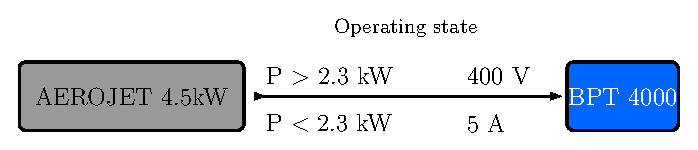
\includegraphics[width=0.4\textwidth]{combination1.eps}}\\
\subbottom[]{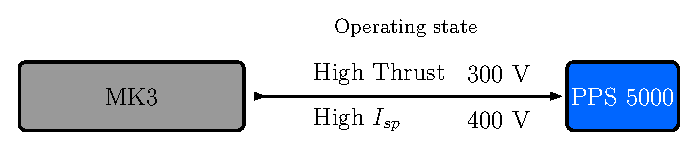
\includegraphics[width=0.4\textwidth]{combination2.eps}}\\
\subbottom[%This is a subfigure\label{fig:label:a}
]{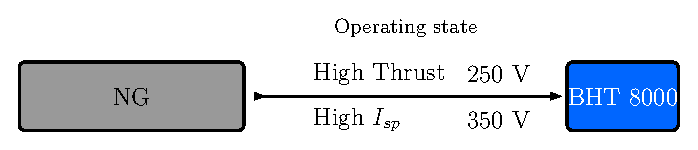
\includegraphics[width=0.4\textwidth]{combination3.eps}}
\caption{\textbf{PPU-HET combinations}}
\label{fig:ppuhetcombinations}
\end{figure}
%
\\The number of thrusters to equip the GEO platform is not a default-option because it depends on the available power from the solar array, as the Solution Path (Sec.\ref{sec:solutionpath}) explains. Consequently, 2 architectures are analyzed for each combination in \figurename\ref{fig:ppuhetcombinations}.
\begin{itemize}
\item Architecture $1$. One nominal thruster, with a Gimbal by Moog$^\copyright$, performs the orbital raising and four  \textit{SPT}-70\footnote{SPT-$70$ belongs to the HET family, so a dedicated PPU is needed. \emph{Xenon} is the propellant.}\cite{}, placed according to the Hispasat \textit{AG1} configuration by OHB System$^\copyright$, are in charge of on-orbit maneuvers. Redundancy is taken into account by doubling the thruster from $\left(1+4\right)$ to $\left(2+8\right)$.
\item Architecture $2$. Two nominal thrusters performs both the orbit raising and the on-orbit maneuvers. They operate synchronously on two deployment mechanisms, following the one described in \cite{corey2010performance}. In order to design a mission as safe as possible, the pair of thruster is doubled, from one per-mechanism to two per-mechanism.
\end{itemize}
The mass budgets ($m_{\scriptstyle{\textsc{sep}}}$) of the six different options (two EP architectures times three HETs) are listed in \tablename\ref{tab:sepmassbudgets}, where other subsystem components are included as well, \textit{i.e.} the Xenon-flow-controller, feeding lines, etc \cite{tesisimo}.
It is worth to specify that the FCT considers that the GEO platform is equipped with only four ($\times~2$ for redundancy) \textit{SPT}-70 for secondary maneuvers, and the burden mass is $60.080~\si{\kilo\gram}$.
%
\begin{table}[htp]
\caption{\textbf{Electric propulsion system mass budgets.}}
\label{tab:electricpropulsionsystemmassbudgets}
\centering
\small
\begin{threeparttable}
\begin{tabular}{lcc}
\toprule
\toprule
HET&$m_{\scriptstyle{\textsc{sep}}}$~Arch. $1^{\star}$&$m_{\scriptstyle{\textsc{sep}}}$~Arch.$2^{\star}$ \\
&$\si{\kilo\gram}$&$\si{\kilo\gram}$\\
\midrule
\textsc{bpt}-$4000$&$128.00$&$121.00$\\
\textsc{pps}-$5000$&$129.40$&$124.60$\\
\textsc{bht}-$8000$&$148.80$&$163.44$\\
\bottomrule
\bottomrule
\end{tabular}
\begin{tablenotes}
\small
\item[$\star$] Added a system margin of $10\%$.
\end{tablenotes}
\end{threeparttable}
\label{tab:sepmassbudgets}
\end{table}
%
\subsection{Chemical Propulsion System}
\label{subsec:chemicalpropulsionsystem}
The chemical propulsion system consists of the components, i.e., engine, tank, valves, feedings and so forth, thus composing the CPM which handles impulsive maneuvers along the CP segment.
A standard bi-propellant system is chosen and it comprises a hypergolic mixture of Monomethylhydrazine (\textit{MMH}) as fuel and Mixed Oxides of Nitrogen ($MON$) or Nitrogen Tetroxide ($N_2O_4$) as oxidizer. The power request from an \textit{AKM} usually is very low (valves, electronics) and it is evaluated around $60~\si{\watt}$, plus a margin of $10\%$. The nominal performances of the selected CP thruster are listed in \tablename\ref{tab:liquidAKM}.
%
\begin{table*}[htp]
\centering
\caption{\textbf{Liquid \textit{AKM}}}
\label{tab:liquidAKM}
\footnotesize
\begin{threeparttable}
\begin{tabular}{*{9}{c}}
\toprule
\toprule
&Fuel/Ox.&$\dfrac{O}{F}$&$T$&$I_{sp}$&$\dot{m}$&$t_{b.o.}$ (tot)&mass\\
&&&$\si{\newton}$&$\si{\second}$&$\si{\kilo\gram\per\second}$&$\si{\hour}$%
&$\si{\kilo\gram}$\\
\midrule
\footnotesize{S400-12}&\footnotesize{MMH/MON}&1.65&420&318&0.135&8.3&3.60\\
\bottomrule
\bottomrule
\end{tabular}
\begin{tablenotes}
\small
\item[$\star$] nominal performance
\item[$\dagger$] From \url{http://www.space-propulsion.com}
\end{tablenotes}
\end{threeparttable}
\end{table*}
%
The CP system is pressurized by Helium; Composite Overwrapped Pressure Vessels (\textit{COPV}s) store the fuel, the oxidizer and the pressurant, and their masses are modeled following the procedure in \citeauthor{wertz2011space}~\cite{wertz2011space}.
\subsubsection{CPM jettisoning}
The detachment of the CPM takes place along the switching orbit and follows the guidelines given by the Inter-Agency Space Debris Coordination Committee \cite{inter2002iadc}.
Based on the position ($r_{jett}$) where the jettisoning is executed ($r_p^s\le r_{jett}\le r_a^s$), there may be several options to choose among:
\begin{itemize}
\item Controlled re-entry;
\item Uncontrolled re-entry in a period lower than 25 years;
\item Storing orbit (e.g. Graveyard);
\end{itemize}
All these alternatives consider the passivization of the CPM, thus all latent energy are depleted. 
\subsection{Power Generation System}
\label{subsec:pgs}
The Power Generations System (PGS) provides, stores, regulates, and distributes electrical power to payloads and other flight subsystems. It is made up of solar solar array, coverglass, batteries and other components. The first two elements are modeled hereinafter, while the batteries, designed to supply energy to the satellite during GEO eclipses, and the harnesses are designed following  standard procedures~\cite{wertz2011space,tesisimo}.
\subsubsection{Solar Array}
\label{subsubsec:solararray}
Solar array (\textit{SA}) is the best solution to provide energy to a satellite for a GEO mission. \emph{The main goal of solar array design for hybrid transfers is to find a proper balance between electric thruster and payload needs}. The introduction of the EP for orbit raising purposes moved the high power request to the SA not only during the GEO parking for the payload's operations, but also along the trajectory path.

If the power P$_{sa}$ \cite{wertz2011space} to size the SA is the same for both the EP segment and the GEO phase, which takes into account also the power to charge the batteries, the PGS will be designed as customized as possible, thus reducing the waste.
This goal is achievable because HETs in \tablename\ref{tab:propertiesofthehetinvestigated} are characterized by a wide operating envelope. Exploiting a power balance process between the aforementioned two power demands~\cite{tesisimo}, the ideal six input powers ($\hat{P}$) during the low-thrust segment for the six EP system combinations are computed as
\begin{equation}
\hat{P} = \mathcal{F}\left(P_{pl}, Architecture,P_{geo-ecl},solar~cell\right)\label{eq:phat}
\end{equation}
where $P_{geo-ecl}$ is the power required from the satellite during the GEO eclipse periods.
The thruster in the Architecture 2 are used at their minimum operating power for the on-orbit maneuvers. Details on the aforementioned method are in \cite{tesisimo}. \tablename\ref{tab:inputpowerofhetfororbitraising} shows the rules to adapt the $\hat{P}$, ideal input power, to the real performances of HET.
%
\begin{table}[htp]
\footnotesize
\centering
\caption{\textbf{Input power of HET for orbit raising}}
\label{tab:inputpowerofhetfororbitraising}
\begin{tabular}{cc}
\toprule
\toprule
Case&Action\\
\midrule
$\hat{P} < P_{MIN}$&$\hat{P}$ is set to $P_{MIN}$\\
$P_{MIN}\le\hat{P}\le P_{MIN}$&$\hat{P}$ is unchanged\\
$\hat{P} < P_{MAX}$&$\hat{P}$ is set to $P_{MAX}$\\
\bottomrule
\bottomrule
\end{tabular}
\end{table}
%
\\
At this point, there are six operating point for the six architectures in terms of thrust, specific impulse and thruster efficiency
\begin{subequations}
\begin{empheq}[left={\empheqlbrace\,}]{align}
T~&=~\mathcal{F_{\scriptstyle\textsc{HET}}}\left(\hat{P},\si{\volt}\right)\label{eq:thrustphat}\\
I_{sp}~&=~\mathcal{G_{\scriptstyle\textsc{HET}}}\left(\hat{P},\si{\volt}\right)\\
\eta~&=~\mathcal{H_{\scriptstyle\textsc{HET}}}\left(\hat{P},\si{\volt}\right)
\end{empheq}
\end{subequations}
where the electrical potential $\si\volt$ correspond to the designed one in \figurename\ref{fig:ppuhetcombinations}.

After this procedure, the user chooses the \emph{mission lifetime in GEO} ($LF_{\textsc{geo}}$) and the desired power life degradation ($L_d=\tfrac{P_{mp}}{P_{mp}}\big|_{\textsc{eol}}$) of the SA at the end-of-life (\textit{EOL}) of the mission, and the SA area is sized following a standard procedure \cite{tesisimo}, where the $P_{sa}$ is the maximum between the power requests during the GEO operations and the orbit raising.

The considered solar cell is the NeXt Triple Junction (\textit{XTJ}) by Spectrolab$^\copyright$ and its performance degradation referred to the 1~$\si{\mega\electronvolt~e}$ electron fluence ($1~\si{\mega\electronvolt~e}$) are outlined in \figurename\ref{fig:powerdegradationofxtjsolarcell}, which is characterized by a linear interpolation
\begin{equation}
\dfrac{P_{mp}}{P_{mp_0}} = \mathcal{F}(\Phi_{1~\si{\mega\electronvolt}}).
\label{eq:xtjphi}
\end{equation} 
obtained from experimental data in \cite{fetzer2008production}.
\begin{figure}[htp]
\centering
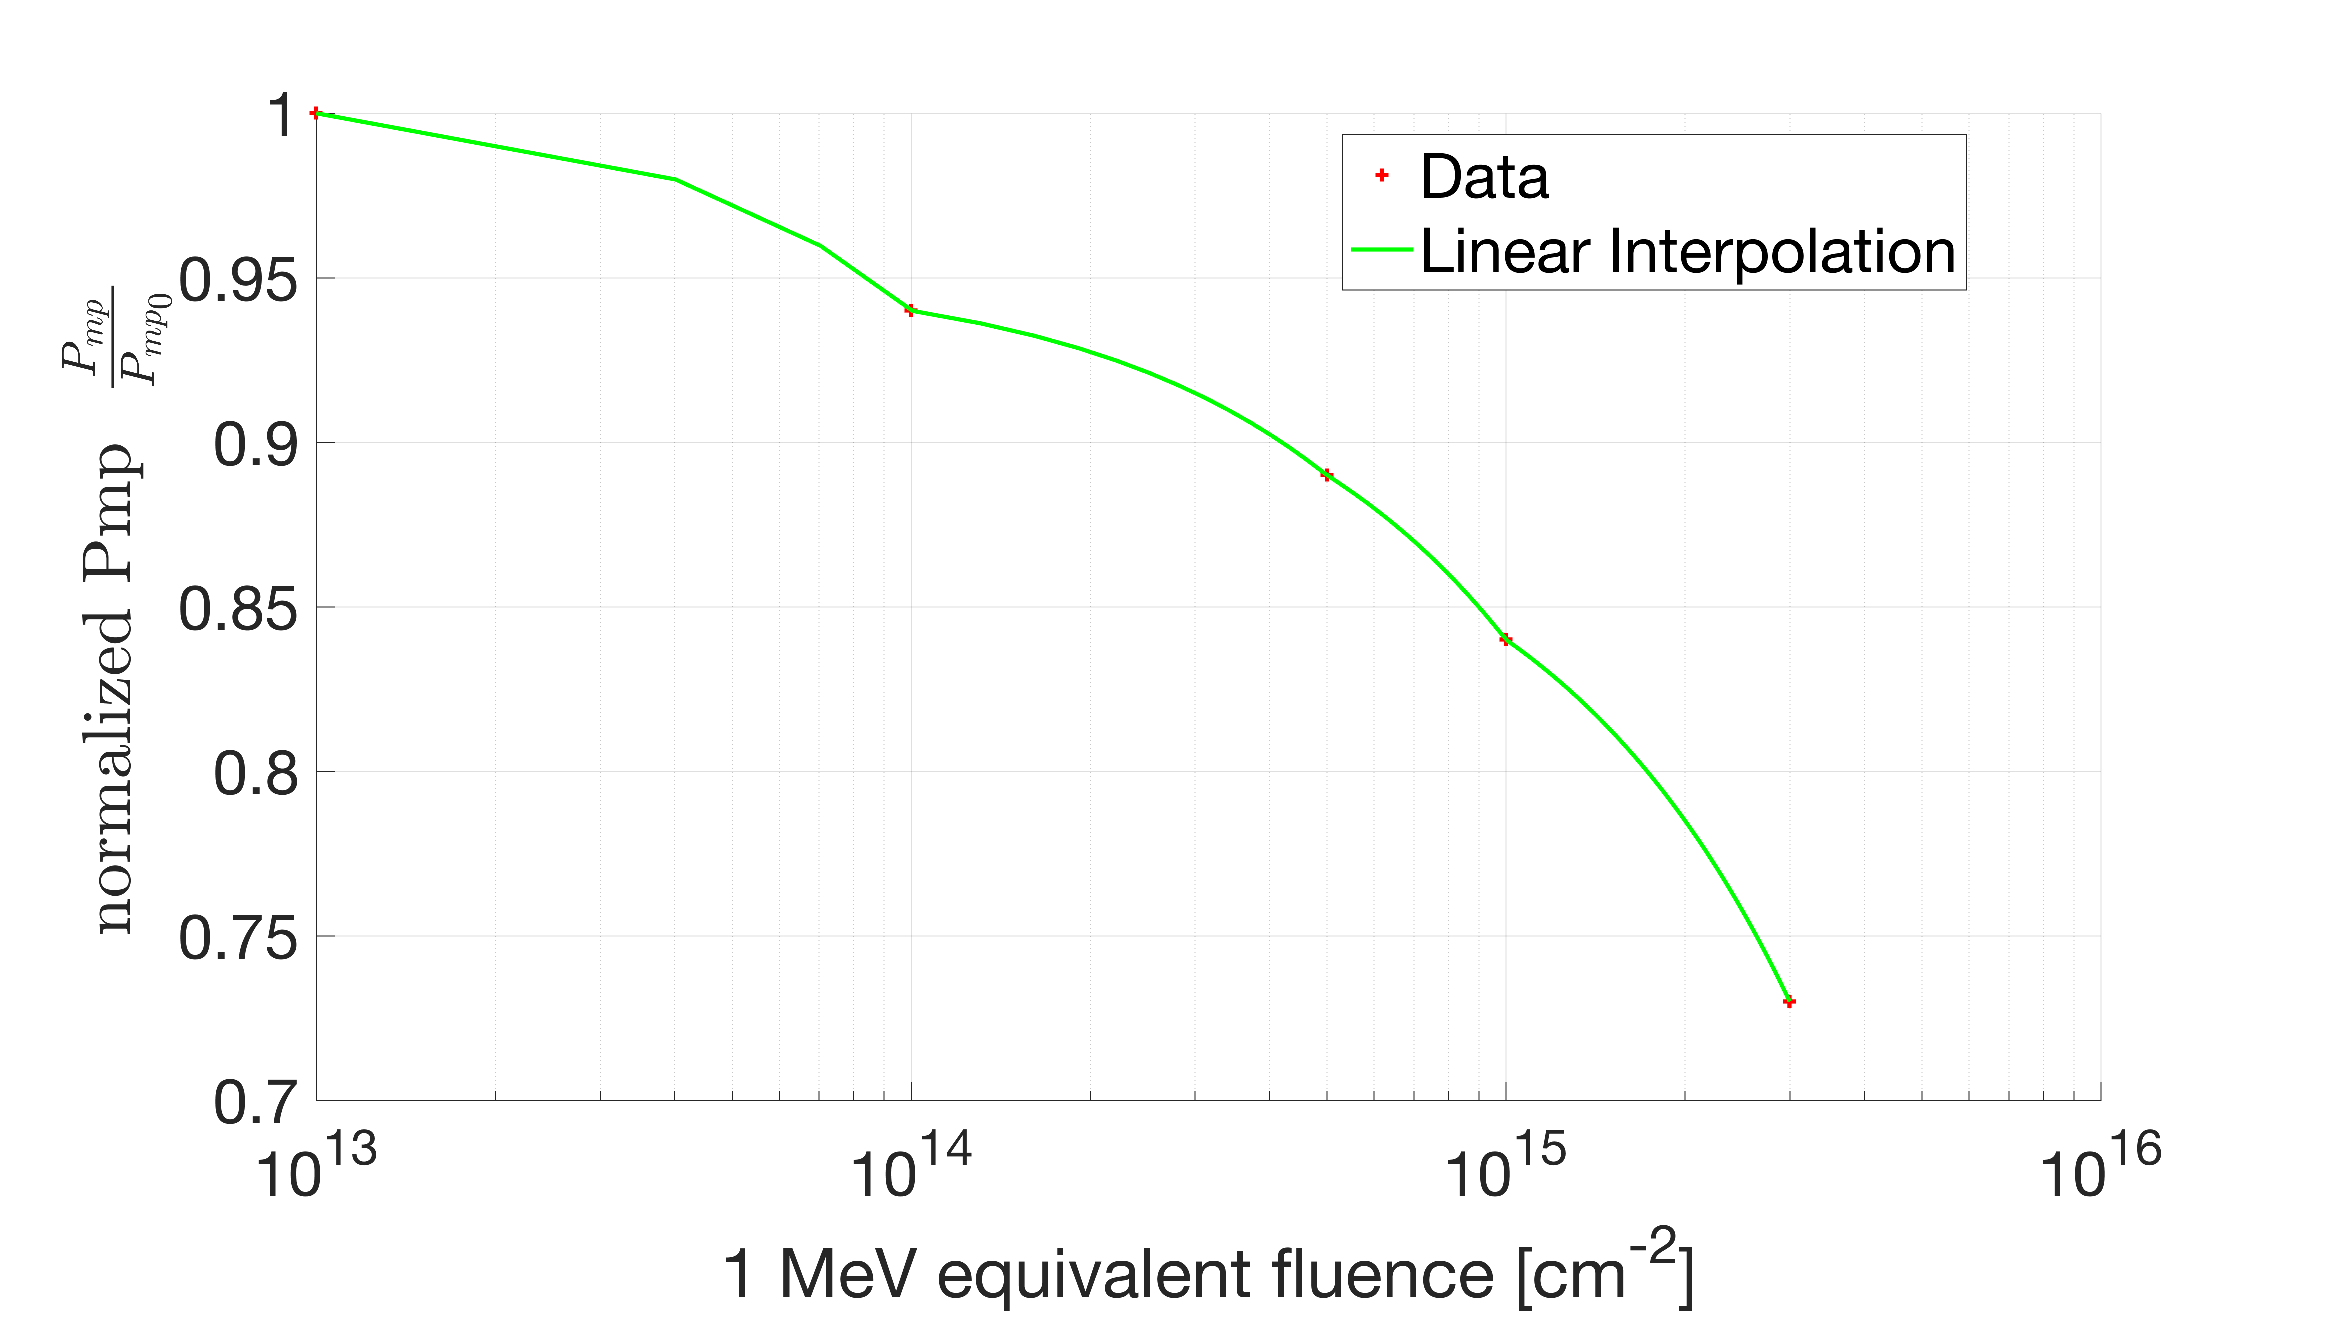
\includegraphics[width=0.45\textwidth]{XTJ_rad.eps}
\caption{\textbf{Power degradation of \textit{XTJ} solar cell.}}
\label{fig:powerdegradationofxtjsolarcell}
\end{figure}
\subsubsection{Coverglass}
The task of the coverglass is to limit the degradation of maximum power generation capability of the solar array, and its thickness $d_{cg}$ is designed in order to meet the requirement on the desired $L_d$ for each HT. Since each HT presents its own path, $d_{cg}$ has not an unique value. This modus operandi allows to consider the power supplied to the SEP constant during the orbit raising, thus supporting the assumption in Sec.\ref{subsubsec:dynamicmodel} about the performances of the thrusters.

It is assumed that Van Allen Belts are the only source of radiations and the CP phase does not count toward radiation absorption. The amount of the total equivalent fluence yields
\begin{equation}
\Phi_{\scriptstyle{1~\si{\mega\electronvolt~e}}}^{\scriptstyle{mission}}~=~\cancelto{0}{\Phi_{\scriptstyle{1~\si{\mega\electronvolt~e}}}^{\scriptstyle{\textsc{CP}}}}+%
\Phi_{\scriptstyle{1~\si{\mega\electronvolt~e}}}^{\scriptstyle{\textsc{EP}}}+%
\Phi_{\scriptstyle{1~\si{\mega\electronvolt~e}}}^{\scriptstyle{\textsc{GEO}}}
\label{eq:radiationcomputation}
\end{equation}
Consequently, the minimum value for $d_{cg}$ corresponds to the GEO mission accomplished by the FCT.

Concerning the evaluation of $\Phi_{1\si{\mega\electronvolt}~e}$ \emph{absorbed during the low-thrust trajectory}, in order to decrease the computational time and to decouple the evaluation from the hybrid transfer analysis, a five dimensional (5-D) table lookup is obtained
%
\begin{equation}
\Phi_{\scriptstyle{1~\si{\mega\electronvolt}}}^{\scriptstyle{\textsc{EP}}} = \mathcal{F}_5\left(R_p, R_a, \dfrac{T}{m_0}, I_{sp}, d_{cg}\right)
\label{eq:fivetablelookup}
\end{equation}
%
where the fifth dimension is the coverglass thickness.
The equivalent fluence data are generated offline. Initially, by running \textit{SPENVIS}$\copyright$\footnote{Data available at \url{http://www.spenvis.oma.be/} [retrieved 1 February 2016].} for a set of circular orbits, thus obtaining the 1-year equivalent fluence data for 8 values of coverglass thickness: d=~$0   , 0.0254, 0.0762, 0.1524, 0.3048, 0.5080,0.7620, 1.5240~\si{\milli\meter}$:
\begin{equation}
\Phi_{\scriptstyle{1~\si{\mega\electronvolt}}}^{\scriptstyle{1year}} = \mathcal{F}\left(R_p, R_a, d_{cg}\right)\label{eq:1yearphi}
\end{equation}
Then, after a procedure detailed in \cite{tesisimo}, $\mathcal{F}_5$ is acquired.